\chapter{Überblick über die Hardware}

Die Motorplatine wurde im Zuge der Studienarbeit von Timo Klingeberg \cite{STUD_TIMO}
entwickelt.
\begin{figure}[htb]
 \centering
 \scalebox{0.5}{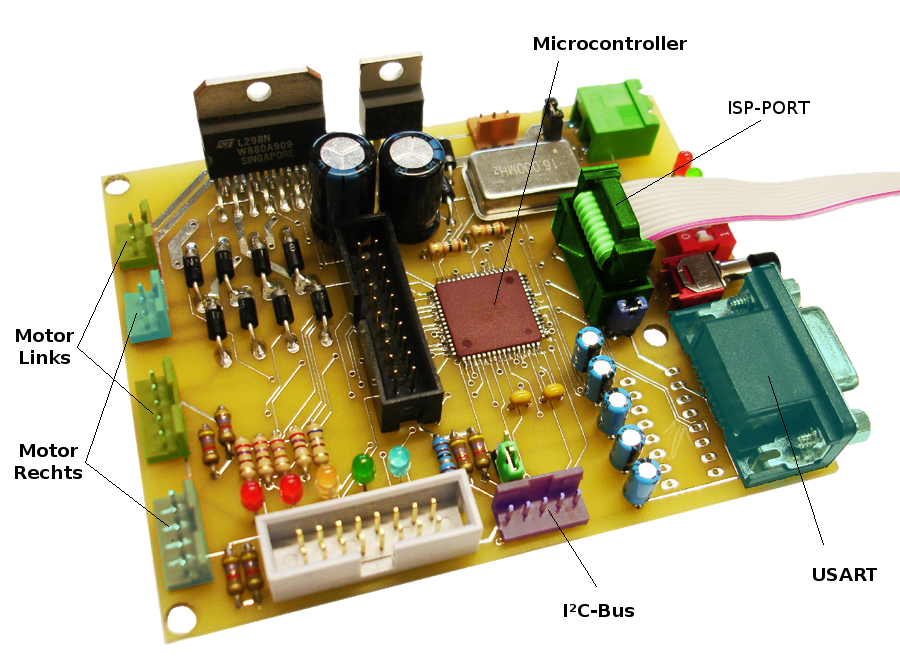
\includegraphics{pictures/board.png}}
 \caption{\label{board}Die Motorplatine}
\end{figure}
\section{Microcontroller}
Das Herzstück der Platine bildet ein Microcontroller der Firma Atmel.
Es handelt sich hierbei um einen ATMEGA2561\cite{ATMEGA_MANUAL}, der 256 KB Speicher für
Programme (Flash) hat, sowie 8 KB Speicher für Variablen (SRAM). Der maximale Takt für
diesen Microcontroller liegt bei 16 MHz, dieser wird auch ausgenutzt. Das bedeutet, dass
ein Takt 62,5 ns benötigt. Da der Großteil der Instruktionen des Microcontrollers nur
einen Takt benötigen, kann er theoretisch 16 MIPS an Leistung erreichen, durch die Benutzung
von Funktionen, Pin-IO und bedingten Sprüngen bleibt dies auch nur eine theoretische Zahl.
Vorteilhafterweise unterstützt der Controller In-System Programming (ISP), was bei der
Entwicklung der Betriebssoftware von großem Nutzen war, da hierdurch schnell und relativ
unkompliziert neue Versionen auf die Platine überspielt werden konnten.\\
Der Controller verfügt über 6 Timer, zwei von diesen sind nur 8-Bit, die anderen vier allerdings
haben 16-Bit, was bei dem gegebenen Takt von 16 MHz einen maximalen Timer-Intervall von 262 ms
entspricht. Zustäzlich kann der Controller sechs Puls-Weiten-Modulationen betreiben, von
denen zwei für die Benutzung der Servomotoren, die die Räder antreiben, benutzt werden.
\section{Ein-/Ausgabemöglichkeiten zur Praktikumsplatine}
Die Motorplatine verfügt sowohl über einen UART-Port, als auch einen I2C-Bus, über die
die Praktikumsplatine mit der Motorplatine kommunizieren kann. Der UART-Port wird außerdem
für die Ausgabe von Debug-Informationen benutzt, falls dies aktiviert wird. Im allgemeinen
Fall wird allerdings nur der I2C-Bus zur Kommunikation zwischen den beiden Platinen verwendet.
Da der Microcontroller über eingebaute Hardwarelogiken sowohl für den I2C-Bus als auch für
den UART-Port verfügt, hält sich der administrative Aufwand für die Kommunikation sehr in
Grenzen. Es können lediglich Interrupt Service Routinen (ISR) für diese zur Verfügung gestellt
werden, die es dann ermöglichen schnell auf Situationen zu reagieren und ohne, dass
Informationen verloren gehen könnten.
\section{Interne Ein-/Ausgabe Ports}
Zusätzlich zu den externen Kommunikationsmöglichkeiten, besitzt der ATMEGA2561 54
programmierbare IO Kanäle, die in Ports mit je 8 Kanälen zusammgefasst werden.
